\paragraph{Decentralized finance.}
We were in the age of centralized infrastructure, where all the ledger states are kept on a centralized node.

\begin{figure}[H]
    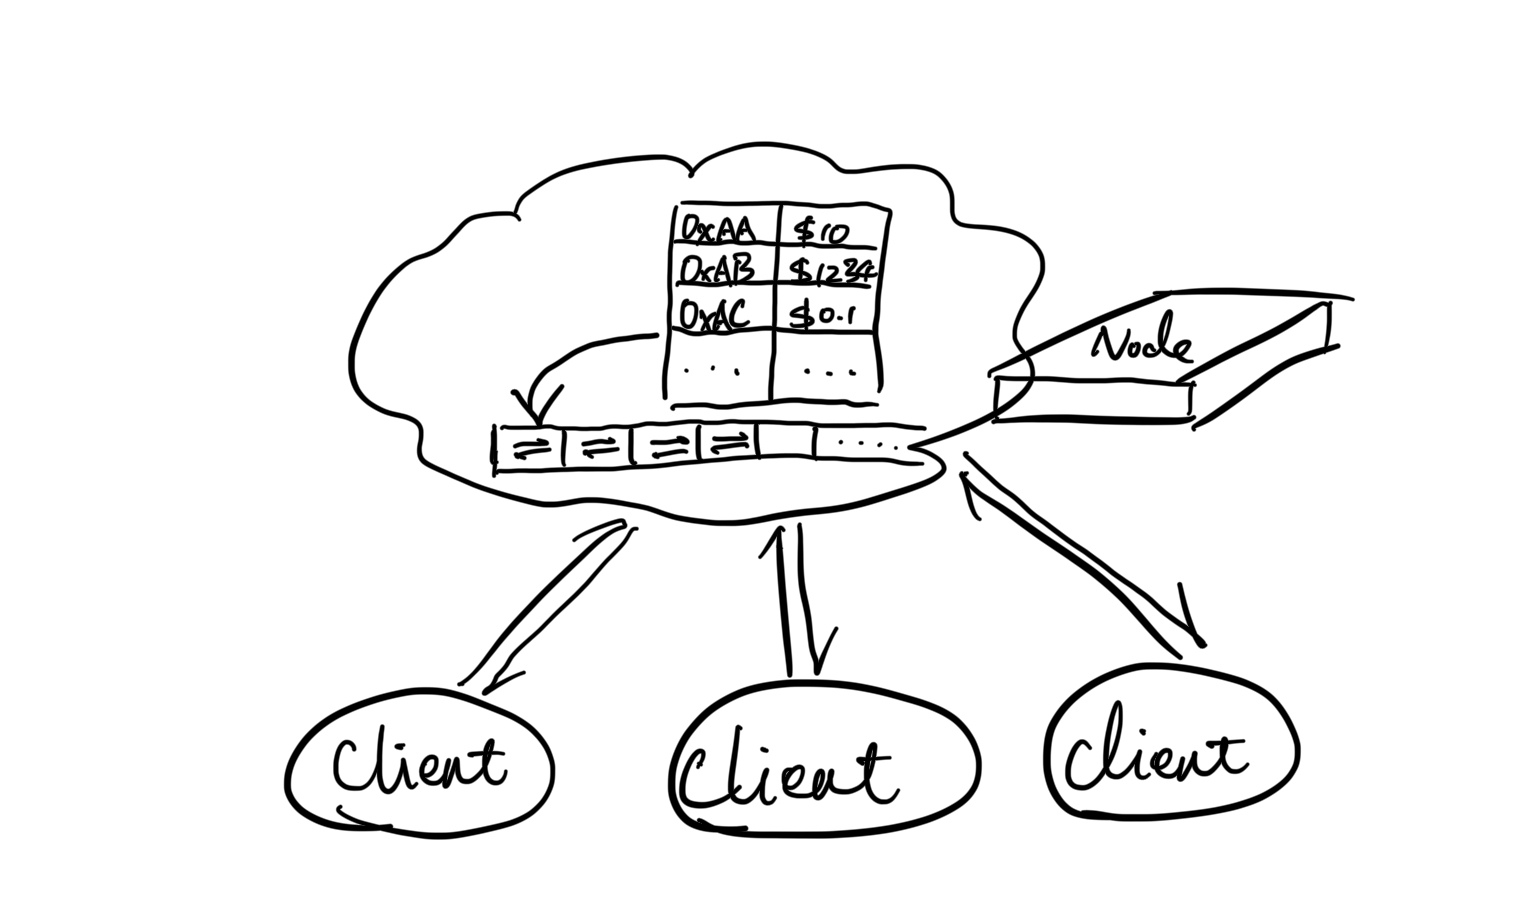
\includegraphics[width=300pt]{graphs/IMG_0050}
    \Description{}
\end{figure}

The upside is the efficiency. Every transition reaches finality in one round trip.
(For bids we consider the finality as the time it is guaranteed to be observable to the other bids.)
Moreover, there's also resource efficiency: the system is running with minimal works being done.
You can literally remove no work but still complete all transactions.
Nothing is wasted.

And the downside has been overly talked.
The centralized operating node can manipulate the market into whatever the node wants it to look like.
Even if directly forging the states can be prohibited (but probably just mitigated) by cryptographic, forging the control path is always doable.
And the most obvious kind of such faults is censorship.

So we move on to the decentralized architecture, prevent single node to have the full control to the ledger.

\begin{figure}[H]
    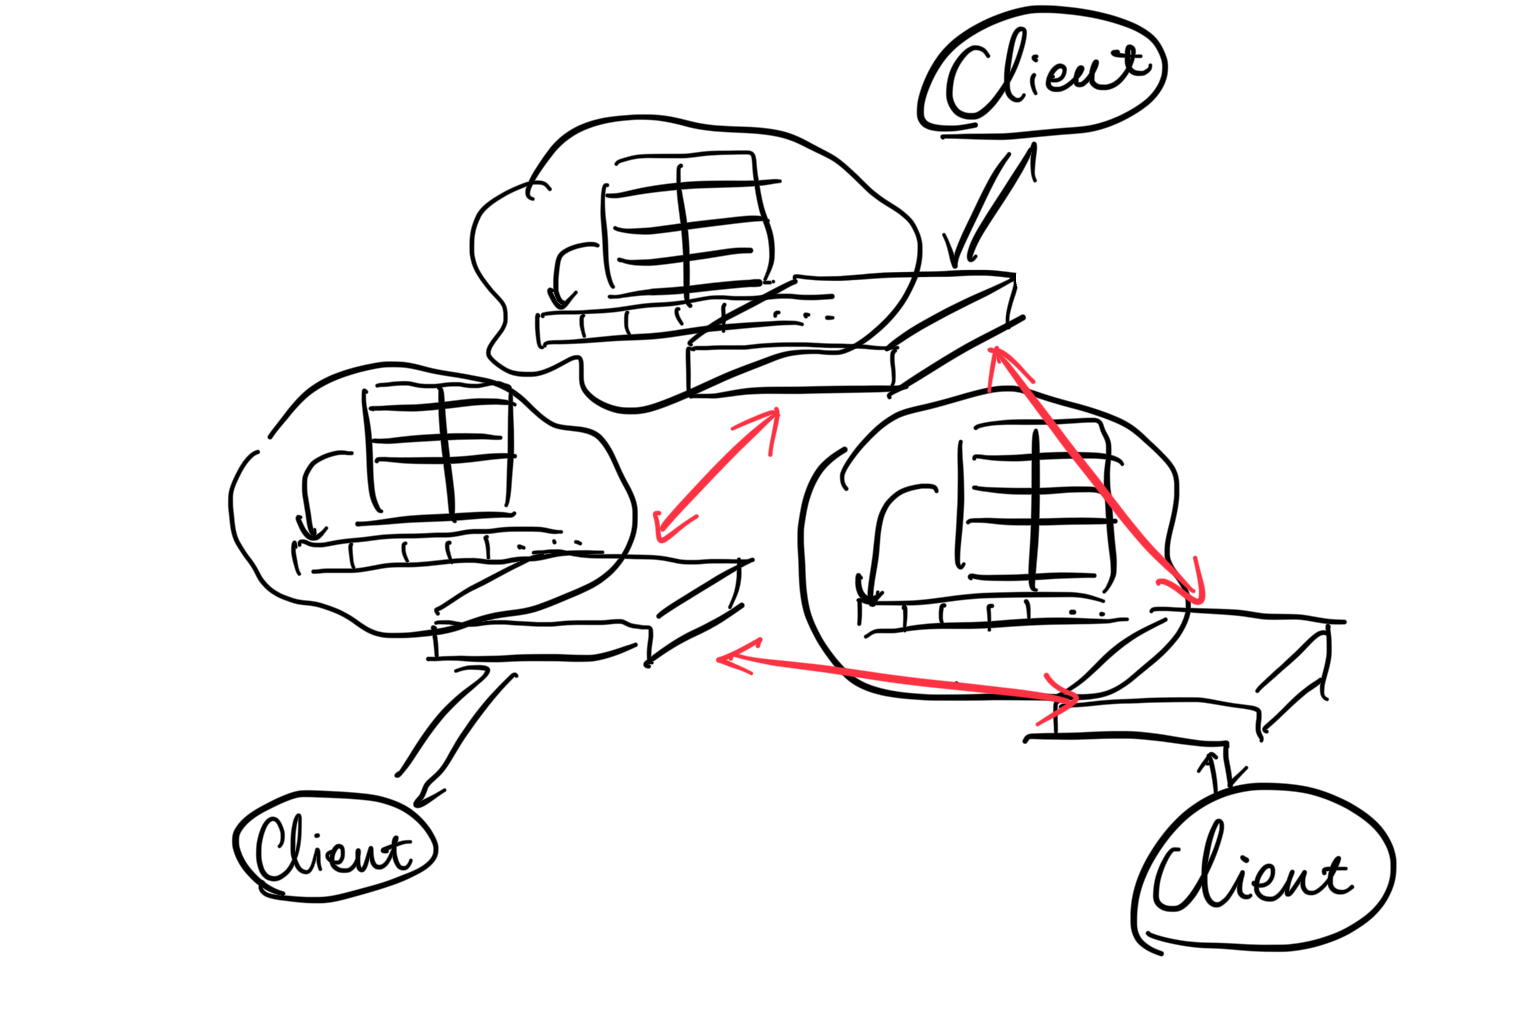
\includegraphics[width=300pt]{graphs/IMG_0051}
    \Description{}
\end{figure}

And we have built a market that cannot be arbitrarily manipulated by (in some definition) minority of the participating powers.

Well, since it's a market it always has some rules.
The rules are usually objective and simple, though you can include a simple ``meta'' rule to allow everyone to add rules so that the running rules may be complicated (but still objective).
The most noticeable property is that all rules \emph{must} be open to everyone.
Only with this property, everyone can \emph{predict} the future ledger states, so they can decide their votes on a candidate running state.

\begin{quote}
    I don't think zero knowledge is changing this fact.
    While ZKP hides some input to the verifier, the logic skeleton is left in the circuit and must be revealed to the public.
    It is theoretically possible to build circuit acting like an interpreter and put the bytecodes into witness, but then the proof probably loses all the security senses.
\end{quote}

\paragraph{Centralized decentralized market.}
But a market that but be predicted into arbitrary future is uninteresting.
And the unpredictable component has been the \emph{proposers}.
Essentially, it has been the proposers who decide the events to be evaluated according the set of predefined rules, and it has been them to decide the future of the market.
Then how are proposers chosen?
Probabilistically toward the most ``powerful'' ones.
So the future of a decentralized market is eventually based on the subjective opinions of the most powerful participants.
This is the root reason for MEV stuff to be possible: subjective opinions matter in the system.

The ``centralized'' decentralized market did not help us go further enough.
While the decentralization can prevent nodes from manipulating markets in the \emph{absolutely} faulty ways, it cannot rule out all self-beneficial attempts.
The control flows are still with (limited) vulnerability.
And it is unsolvable with the ``define the rules and everyone follows'' approach as long as your rules do not lead to a deterministic future, which is the basic requirement for any useful system (except the ones solving scientific puzzles).

The root cause of such undesirable centralization is the fact that everyone is sharing the same mutable states.

\begin{figure}[H]
    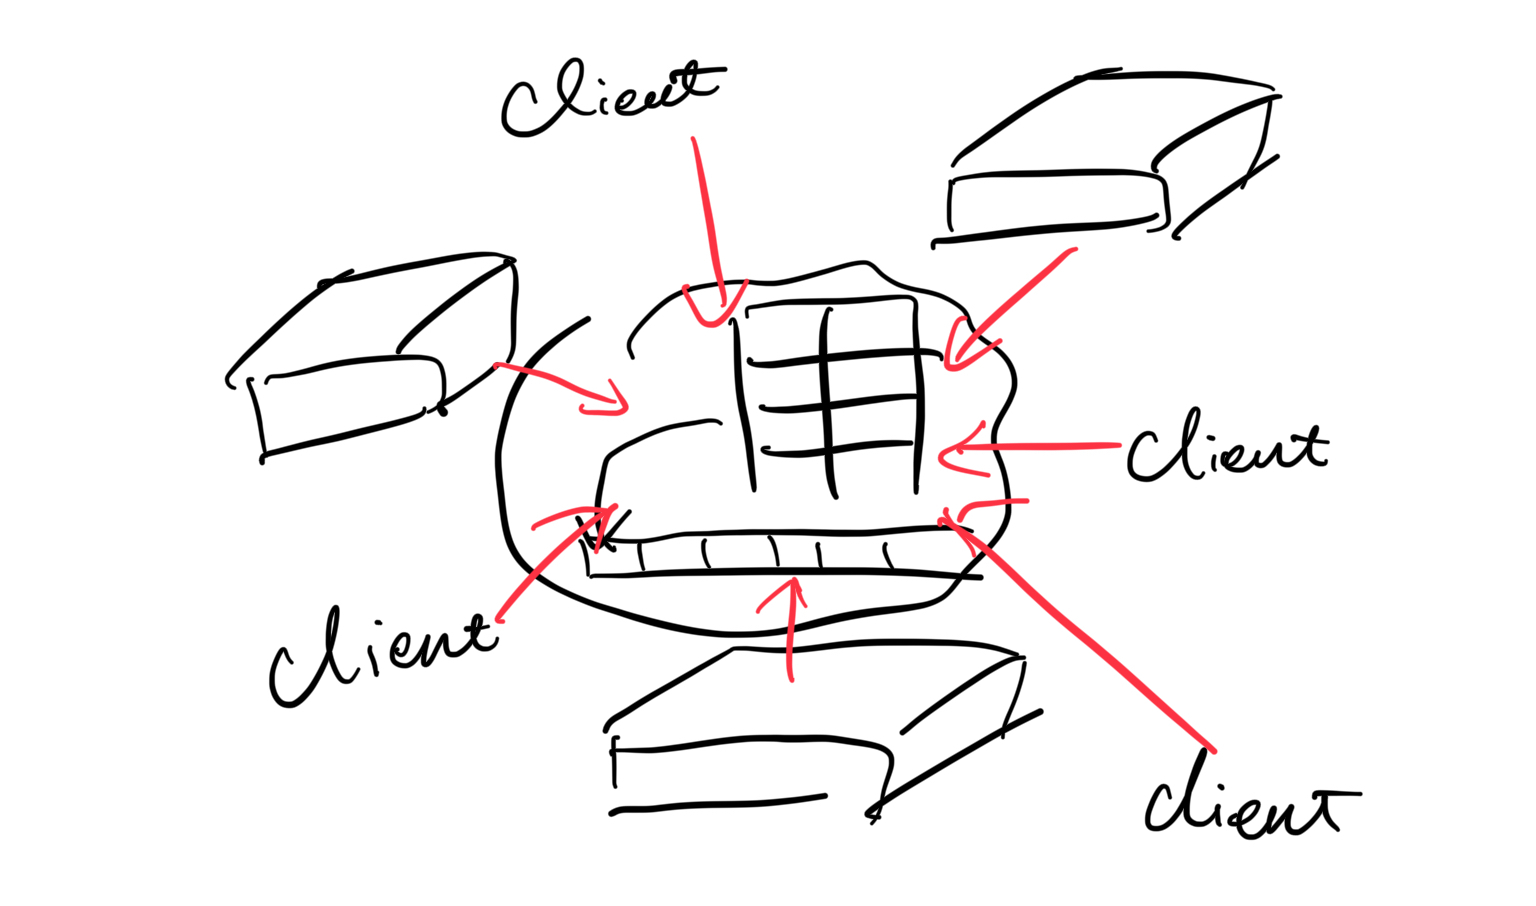
\includegraphics[width=300pt]{graphs/IMG_0061}
    \Description{}
\end{figure}

And every mutation of the states must be initiated by \emph{someone}, instead of objective rules, to enable unpredictable markets.

The current mitigation is to randomize the proposers.
This approach trades security with performance.
The large scope of candidate proposers of a round, the more overhead.
This is a solution that cannot scale.
Moreover, considering we have already traded a lot of performance for just propagating the shared state globally, this approach push us even further from the centralized markets in the sense of performance metrics.
The quantitative differences eventually lead to substantial ones.
There are certain services that widely provided by centralized markets, while impractical/not meaningful as smart contracts because of the poor performance.

Consensus drags.